\section{Structure from Motion}

We ran experiments with 3 different keypoint detectors (a frame of the video is shown in figure \ref{fig:final-tracking}) and this give as an idea of the best number of keypoints. As can be seen in figure \ref{fig:comparison-keypoints-sfm}.b, if the number of keypoints is low, it is difficult to notice the form, while if we consider more points (SIFT may consider foreground points) we can create some noise that is not desirable (figure \ref{fig:comparison-keypoints-sfm}.c), on the other hand, considering a lot of points but in specific parts of the object (specially in the borders) give us a better understanding of the structure (figure \ref{fig:comparison-keypoints-sfm}.a). Hence, a lot of points are desirable but their location is also important for better reconstruction.

\begin{figure}[H]
	\centering
	\begin{subfigure}{0.5\textwidth}
	  \centering
	  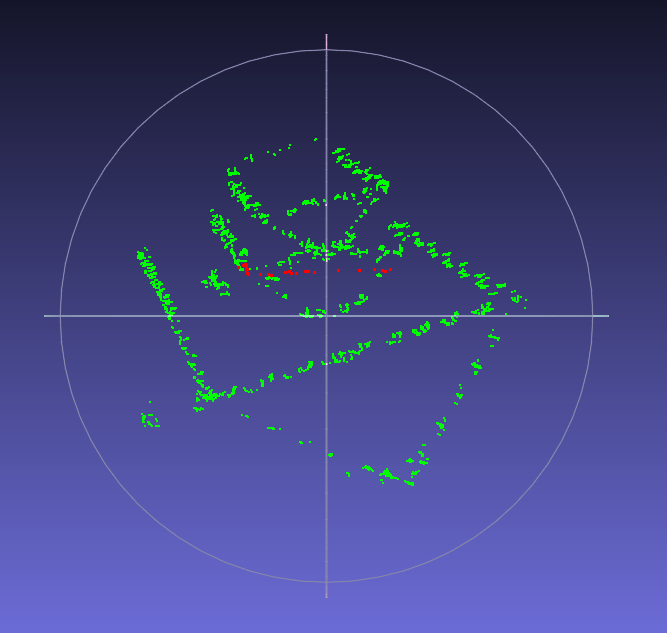
\includegraphics[width=0.9\linewidth]{figs/SFM1.png}
	  \caption{Harris}
	\end{subfigure}%
	\begin{subfigure}{0.5\textwidth}
	  \centering
	  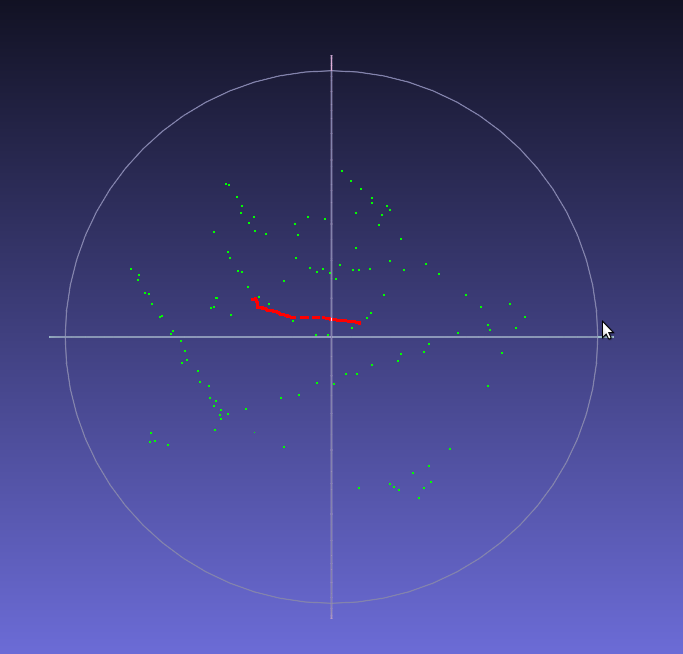
\includegraphics[width=0.9\linewidth]{figs/SFM1-Shitomosi.png}
	  \caption{Shi-Tomasi}
	\end{subfigure}
	\begin{subfigure}{0.5\textwidth}
        \centering
        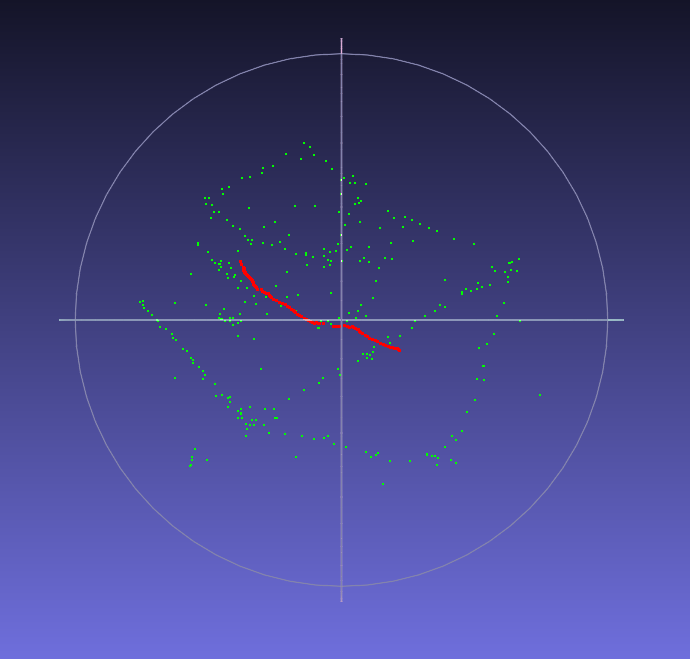
\includegraphics[width=0.9\linewidth]{figs/SFM1-sift.png}
        \caption{SIFT}
      \end{subfigure}
       \caption{Comparison of Structure from motion with different keypoint detectors.}
	\label{fig:comparison-keypoints-sfm}
\end{figure}

Results of the structure from motion are shown in figure \ref{fig:sfm}, note that the structure is represented by green points and the camera path with red points.

\begin{figure}[H]
	\centering
	\begin{subfigure}{0.5\textwidth}
	  \centering
	  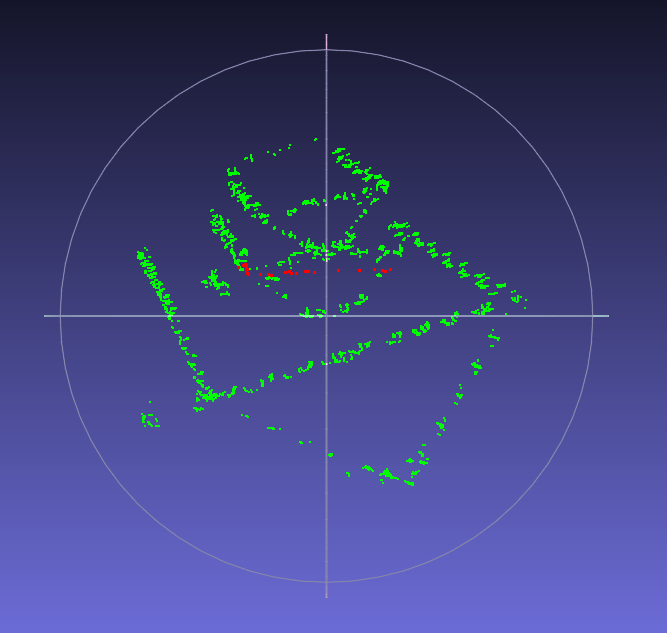
\includegraphics[width=0.9\linewidth]{figs/SFM1.png}
	\end{subfigure}%
	\begin{subfigure}{0.5\textwidth}
	  \centering
	  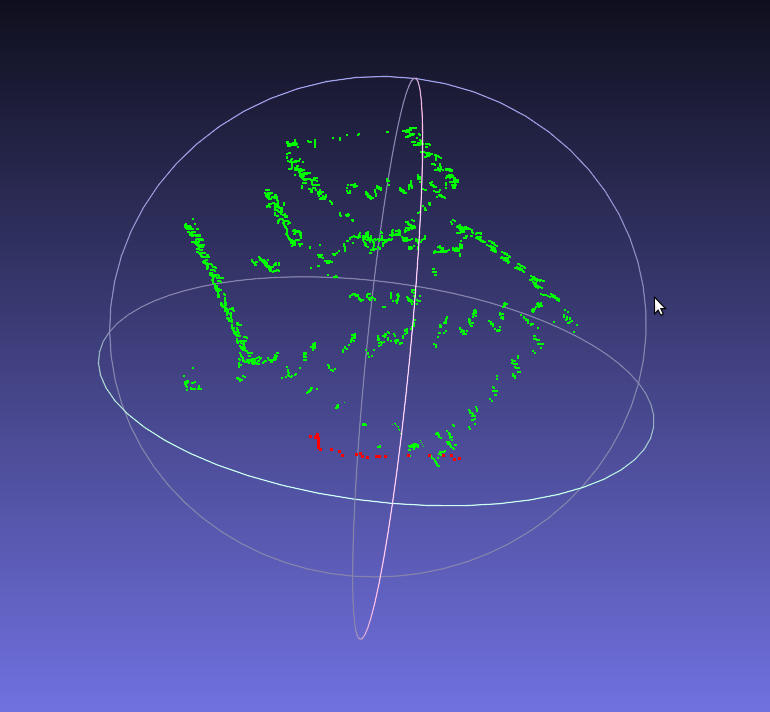
\includegraphics[width=0.9\linewidth]{figs/SFM2.png}
	\end{subfigure}
	\begin{subfigure}{0.5\textwidth}
      \centering
      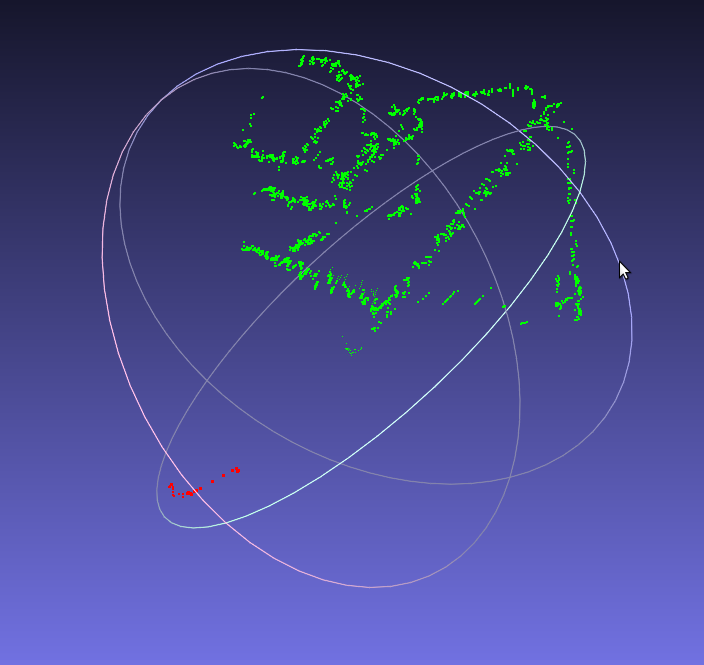
\includegraphics[width=0.9\linewidth]{figs/SFM3.png}
    \end{subfigure}
    \caption{Structure from motion with Harris detector.}
	\label{fig:sfm}
\end{figure}


The expected technique to recover the camera position is to use homogeneous coordinates in the equation $X = MS$, such that when solving this system, $M$ represents a transformation sub matrixes $m$ of size $3 \times 4$ that maps a 3D point $(X, Y, Z, 1)$ to a 2D point $(x, y, 1)$, then $m$ can be expressed as $[C R]$ where $C$ is a $3 \times 3$ and $R = -CP$ is $3 \times 1$, then, the camera position $P$ can be computed as $-C^{-1} R$, but we had problems working with homogeneous coordinates when solving with Cholesky decomposition(not positive definite matrix as input), we think this is because when constructing $X$ in homogeneous coordinates and filling a third of the matrix with 1's the rank of the matrix remains three and the intermediate results rich in a non positive definite matrix, thus in order to recover the camera path we work over the $2\times 3$ matrix $m$ without homogeneous coordinates, let $m = \begin{bmatrix}
    m_{11} & m_{12} & m_{13} \\
    m_{21} & m_{22} & m_{23} 
\end{bmatrix}
$, then the camera position is given by the cross-product of vectors $[m_{11}, m_{12}, m_{13}]$ and  $[m_{21}, m_{22}, m_{23}]$, the reason we use this product is that if the image plane is orthogonal to a vector $V$ that goes from the origin of the 3D world \footnote{Note that center of the 3D world is also the centroit of the 3D object (assumtion of Factorization method)} and  $[m_{11}, m_{12}, m_{13}]$, $[m_{21}, m_{22}, m_{23}]$ defines the image plane, then, its cross product is also orthogonal to the image plane. The magnitude of this cross product is usually small, thus we multiply the result by a constant (experimentally setted to 200) before plotting.




